% -*- Mode:TeX -*-

%% IMPORTANT: The official thesis specifications are available at:
%%            http://libraries.mit.edu/archives/thesis-specs/
%%
%%            Please verify your thesis' formatting and copyright
%%            assignment before submission.  If you notice any
%%            discrepancies between these templates and the 
%%            MIT Libraries' specs, please let us know
%%            by e-mailing thesis@mit.edu

%% The documentclass options along with the pagestyle can be used to generate
%% a technical report, a draft copy, or a regular thesis.  You may need to
%% re-specify the pagestyle after you \include  cover.tex.  For more
%% information, see the first few lines of mitthesis.cls. 

%\documentclass[12pt,vi,twoside]{mitthesis}
%%
%%  If you want your thesis copyright to you instead of MIT, use the
%%  ``vi'' option, as above.
%%
%\documentclass[12pt,twoside,leftblank]{mitthesis}
%%
%% If you want blank pages before new chapters to be labelled ``This
%% Page Intentionally Left Blank'', use the ``leftblank'' option, as
%% above. 

\documentclass[11pt,oneside]{mitthesis}
\usepackage{lgrind}
\usepackage{titlesec}
\usepackage{pgfplots}
\usepackage{listings}
\usepackage{pdfpages}
\lstset{language=C}
\usepackage{nomencl}
\usepackage{siunitx}

\usepackage{float}

\usepackage[europeanresistors]{circuitikz}

\usepackage{tikz}
%% These have been added at the request of the MIT Libraries, because
%% some PDF conversions mess up the l50\,$\mu$migatures.  -LB, 1/22/2014
\usepackage{cmap}
\usepackage[T1]{fontenc}
\usepackage[utf8]{inputenc}
\pgfplotsset{every axis legend/.append style={
at={(1.1,0.2)},
anchor=south west}} 


\pagestyle{plain}
\titlespacing\section{0pt}{12pt plus 4pt minus 2pt}{12pt plus 4pt minus 8pt}
\renewcommand{\chaptername}{Kapitola}
\renewcommand{\figurename}{Obrázek}
\renewcommand{\tablename}{Tabulka}
\renewcommand{\contentsname}{Obsah}
\renewcommand{\contentsname}{Obsah}
\renewcommand{\listtablename}{Tabulky}
\renewcommand{\listfigurename}{Obrázky}
\renewcommand\bibname{Reference}

%\addtocontents{toc}{\protect\thispagestyle{empty}}
%\addtocontents{lof}{\protect\thispagestyle{empty}}

\newcommand{\itab}[1]{\hspace{0em}\rlap{#1}}
\newcommand{\tab}[1]{\hspace{.2\textwidth}\rlap{#1}}

\newcommand\uv[1]{\quotedblbase #1\textquotedblleft}
\usepgfplotslibrary{polar}
\makenomenclature

\begin{document}

% -*-latex-*-
% 
% For questions, comments, concerns or complaints:
% thesis@mit.edu
% 
%
% $Log: cover.tex,v $
% Revision 1.8  2008/05/13 15:02:15  jdreed
% Degree month is June, not May.  Added note about prevdegrees.
% Arthur Smith's title updated
%
% Revision 1.7  2001/02/08 18:53:16  boojum
% changed some \newpages to \cleardoublepages
%
% Revision 1.6  1999/10/21 14:49:31  boojum
% changed comment referring to documentstyle
%
% Revision 1.5  1999/10/21 14:39:04  boojum
% *** empty log message ***
%
% Revision 1.4  1997/04/18  17:54:10  othomas
% added page numbers on abstract and cover, and made 1 abstract
% page the default rather than 2.  (anne hunter tells me this
% is the new institute standard.)
%
% Revision 1.4  1997/04/18  17:54:10  othomas
% added page numbers on abstract and cover, and made 1 abstract
% page the default rather than 2.  (anne hunter tells me this
% is the new institute standard.)
%
% Revision 1.3  93/05/17  17:06:29  starflt
% Added acknowledgements section (suggested by tompalka)
% 
% Revision 1.2  92/04/22  13:13:13  epeisach
% Fixes for 1991 course 6 requirements
% Phrase "and to grant others the right to do so" has been added to 
% permission clause
% Second copy of abstract is not counted as separate pages so numbering works
% out
% 
% Revision 1.1  92/04/22  13:08:20  epeisach

% NOTE:
% These templates make an effort to conform to the MIT Thesis specifications,
% however the specifications can change.  We recommend that you verify the
% layout of your title page with your thesis advisor and/or the MIT 
% Libraries before printing your final copy.

\title{Trychtýřová anténa s dielektrickou čočkou realizovaná technologií 3D tisku}

\author{Michal Průša}
% If you wish to list your previous degrees on the cover page, use the 
% previous degrees command:
%       \prevdegrees{A.A., Harvard University (1985)}
% You can use the \\ command to list multiple previous degrees
%       \prevdegrees{B.S., University of California (1978) \\
%                    S.M., Massachusetts Institute of Technology (1981)}
\department{katedra elektromagnetického pole}

\Work{Diplomová práce}
\WORK{DIPLOMOVÁ PRÁCE}

\FACULTY{FAKULTA ELEKTROTECHNICKÁ}
\faculty{fakulta elektrotechnická}
%\faculty{fakulta elektrotechnická}
% If the thesis is for two degrees simultaneously, list them both
% separated by \and like this:
% \degree{Doctor of Philosophy \and Master of Science}
\degree{Bakalar}

% As of the 2007-08 academic year, valid degree months are September, 
% February, or June.  The default is June.
\degreemonth{Květen}
\degreeyear{2017}
\thesisdate{May 20, 2017}

%% By default, the thesis will be copyrighted to MIT.  If you need to copyright
%% the thesis to yourself, just specify the `vi' documentclass option.  If for
%% some reason you want to exactly specify the copyright notice text, you can
%% use the \copyrightnoticetext command.  
%\copyrightnoticetext{\copyright IBM, 1990.  Do not open till Xmas.}

% If there is more than one supervisor, use the \supervisor command
% once for each.
\supervisor{Ing. Tomáš Kořínek PhD.}
% This is the department committee chairman, not the thesis committee
% chairman.  You should replace this with your Department's Committee
% Chairman.
\chairman{Arthur C. Smith}{Chairman, Department Committee on Graduate Theses}

% Make the titlepage based on the above information.  If you need
% something special and can't use the standard form, you can specify
% the exact text of the titlepage yourself.  Put it in a titlepage
% environment and leave blank lines where you want vertical space.
% The spaces will be adjusted to fill the entire page.  The dotted

\makecover
% lines for the signatures are made with the \signature command.

\thispagestyle{empty}
\null\newpage
\maketitle

\cleardoublepage
\thispagestyle{empty}
\section*{Čestné prohlášení}

% $Log: abstract.tex,v $
% Revision 1.1  93/05/14  14:56:25  starflt
% Initial revision
% 
% Revision 1.1  90/05/04  10:41:01  lwvanels
% Initial revision
% 
%
%% The text of your abstract and nothing else (other than comments) goes here.
%% It will be single-spaced and the rest of the text that is supposed to go on
%% the abstract page will be generated by the abstractpage environment.  This
%% file should be \input (not \include 'd) from cover.tex.
Prohlašuji, že jsem zadanou bakalářskou práci „Trychtýřová anténa s dielektrickou čočkou realizovaná technologií 3D tisku“ zpracoval sám s přispěním vedoucího práce a používal jsem pouze literaturu uvedenou na konci práce. Souhlasím se zapůjčováním práce a jejím zveřejňováním.
\vspace{2cm}

\noindent V Praze dne 18.5.2017 \hfill Michal Průša


\cleardoublepage

% $Log: abstract.tex,v $
% Revision 1.1  93/05/14  14:56:25  starflt
% Initial revision
% 
% Revision 1.1  90/05/04  10:41:01  lwvanels
% Initial revision
% 
%
%% The text of your abstract and nothing else (other than comments) goes here.
%% It will be single-spaced and the rest of the text that is supposed to go on
%% the abstract page will be generated by the abstractpage environment.  This
%% file should be \input (not \include 'd) from cover.tex.

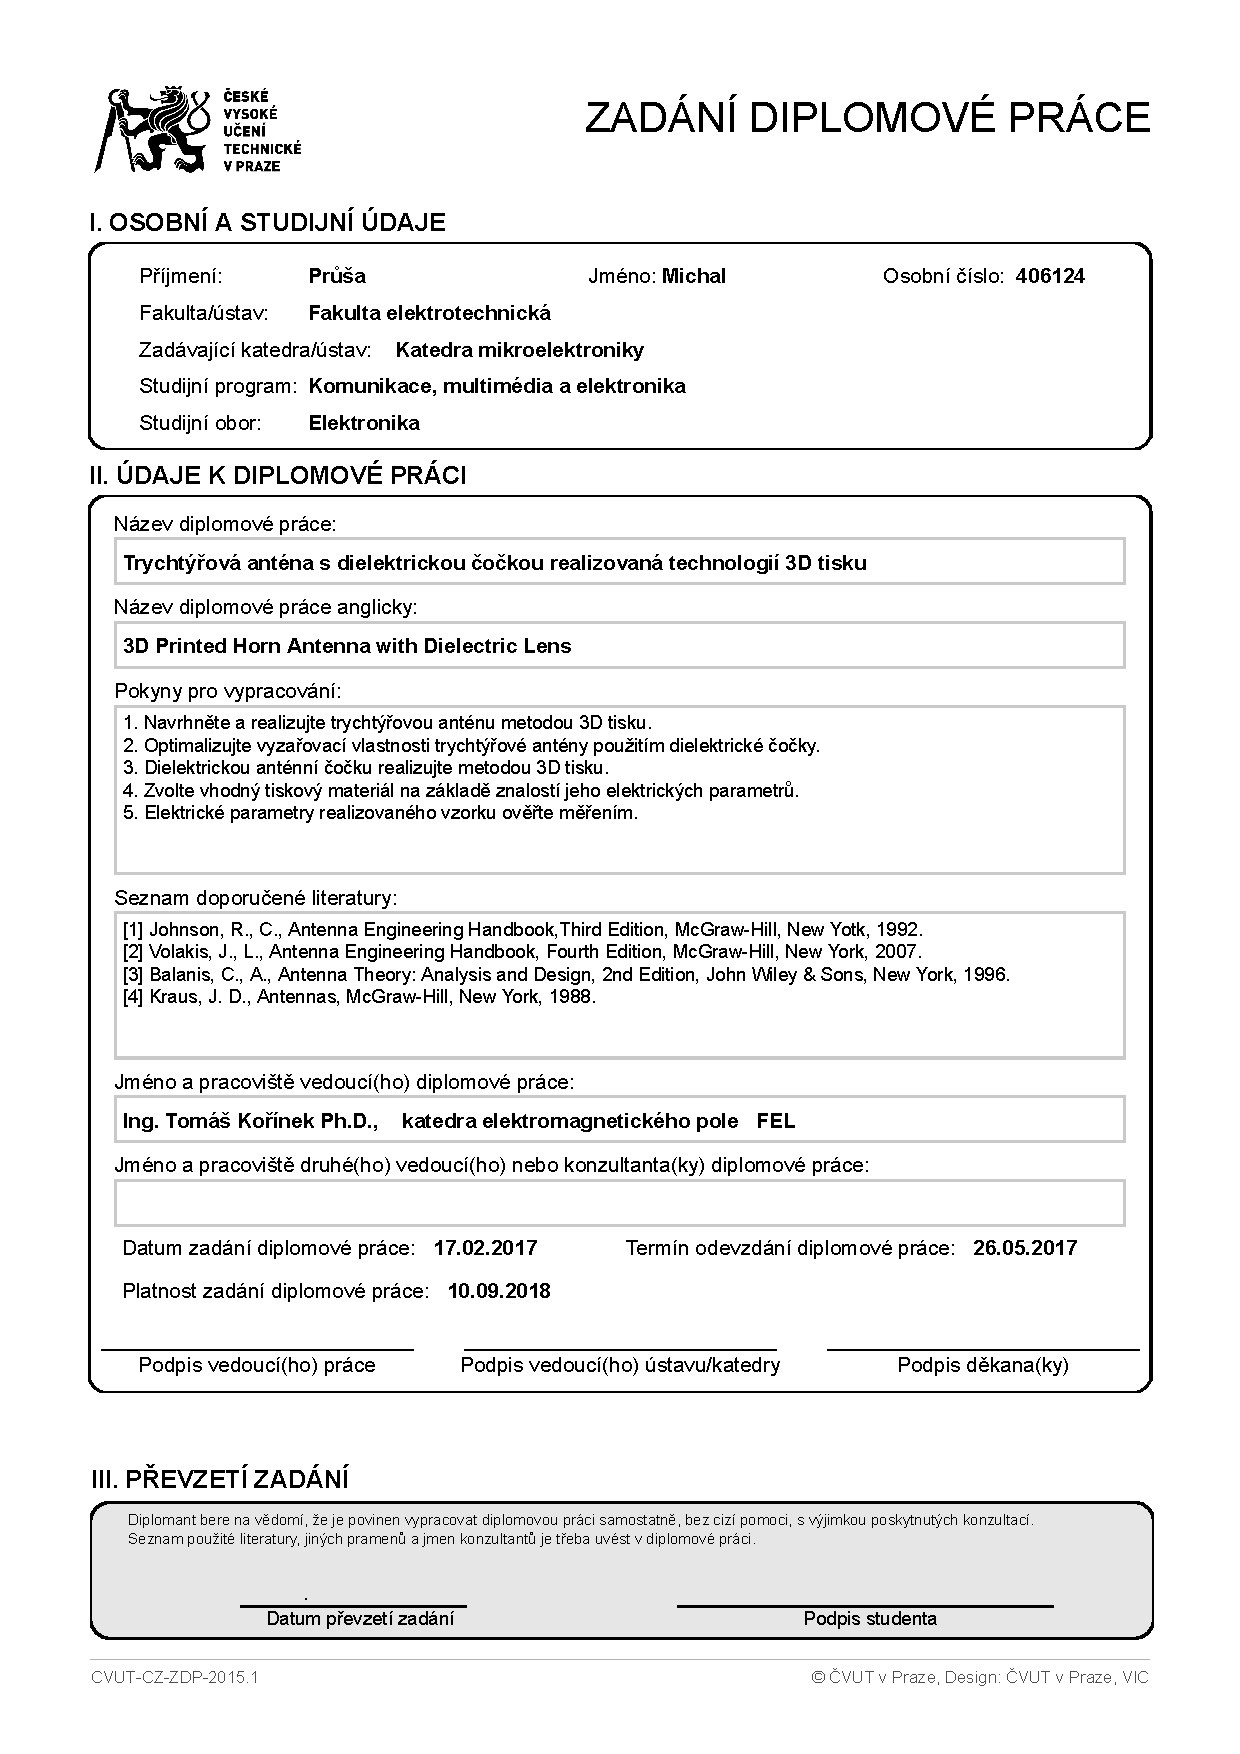
\includepdf[pages={1}]{zadani-nosign.pdf}


\cleardoublepage


\cleardoublepage
\thispagestyle{empty}
\section*{Poděkování}

% $Log: abstract.tex,v $
% Revision 1.1  93/05/14  14:56:25  starflt
% Initial revision
% 
% Revision 1.1  90/05/04  10:41:01  lwvanels
% Initial revision
% 
%
%% The text of your abstract and nothing else (other than comments) goes here.
%% It will be single-spaced and the rest of the text that is supposed to go on
%% the abstract page will be generated by the abstractpage environment.  This
%% file should be \input (not \include 'd) from cover.tex.
Mé poděkování patří panu Ing. Tomášovi Kořínkovi PhD. za cenné rady při konzultacích, za podporu, ochotu, vstřícnost a trpělivost při vedení celé této diplomové práce.

Dále mé poděkování patří firmě Prusa Research s.r.o. za poskytnutí tiskové laboratoře a finančních prostředků.


% The abstractpage environment sets up everything on the page except
% the text itself.  The title and other header material are put at the
% top of the page, and the supervisors are listed at the bottom.  A
% new page is begun both before and after.  Of course, an abstract may
% be more than one page itself.  If you need more control over the
% format of the page, you can use the abstract environment, which puts
% the word "Abstract" at the beginning and single spaces its text.

%% You can either \input (*not* \include) your abstract file, or you can put
%% the text of the abstract directly between the \begin{abstractpage} and
%% \end{abstractpage} commands.

% First copy: start a new page, and save the page number.
\cleardoublepage
% Uncomment the next line if you do NOT want a page number on your
% abstract and acknowledgments pages.
% \pagestyle{empty}

\thispagestyle{empty}
% $Log: abstract.tex,v $
% Revision 1.1  93/05/14  14:56:25  starflt
% Initial revision
% 
% Revision 1.1  90/05/04  10:41:01  lwvanels
% Initial revision
% 
%
%% The text of your abstract and nothing else (other than comments) goes here.
%% It will be single-spaced and the rest of the text that is supposed to go on
%% the abstract page will be generated by the abstractpage environment.  This
%% file should be \input (not \include 'd) from cover.tex.

\section*{Anotace}

Obsahem této diplomové práce je výhradně rozbor využití FDM/FFF technologie 3D tisku ve vysokofrekvenční technice, konkrétně možnosti realizace trychtýřové antény s dielektrickou čočkou pro optimalizaci vyzařovacích vlastností. V první části se práce zabývá trychtýřovými anténami a jejich návrhem, následně stejným postupem dielektrickými čočkami. Dále se práce zabývá materiály pro 3D tisk, jejich parametry, včetně extrakce a popisu metody. Závěrem práce je popis realizace navržené antény, předvedeny výsledky a porovnány se simulací.
Postupy popsanými v této práci se podařilo realizovat funkční trychtýřovou anténu s dielektrickou čočkou pomocí 3D tisku, bohužel s velmi nízkým ziskem, a extrahovat parametry běžných materiálů po průchodu procesem.


\section*{Klíčová slova}

3D tisk, RepRap, Trychtýřová anténa, Anténní čočka, Dielektrická čočka, Extrakce parametrů

\section*{Abstract}

Content of this masters thesis is specially a research of possible usage of FDM/FFF 3D printing technology in high frequency technology, specifically realization of horn antenna with dielectric lens for optimization of radiation properties. In the first part, the thesis is explaining horn antennas and it's design, then dielectric lenses in similar way. Then the materials for 3D printing is discussed, described properties and it's extraction, including description of the method. At the end, realization of designed antenna and lens is described, presented results and compared to simulation.
With methods described in this thesis, we were able to realize working horn antenna with dielectric lens using 3D printing technology, unfortunately with very low gain, and extract parameters of common materials after printing process.


\section*{Key words}

3D printer, RepRap, Horn antenna, Antenna lens, Dielectric lens, Parameter Extraction


% Additional copy: start a new page, and reset the page number.  This way,
% the second copy of the abstract is not counted as separate pages.
% Uncomment the next 6 lines if you need two copies of the abstract
% page.
% \setcounter{page}{\thesavepage}
% \begin{abstractpage}
% \input{abstract}
% \end{abstractpage}
\setcounter{savepage}{\thepage}
\cleardoublepage



%%%%%%%%%%%%%%%%%%%%%%%%%%%%%%%%%%%%%%%%%%%%%%%%%%%%%%%%%%%%%%%%%%%%%%
% -*-latex-*-



\pagestyle{plain}
  % -*- Mode:TeX -*-
%% This file simply contains the commands that actually generate the table of
%% contents and lists of figures and tables.  You can omit any or all of
%% these files by simply taking out the appropriate command.  For more
%% information on these files, see appendix C.3.3 of the LaTeX manual. 
\thispagestyle{empty}
\tableofcontents
\thispagestyle{empty}



\setcounter{page}{1}
%% This is an example first chapter.  You should put chapter/appendix that you
%% write into a separate file, and add a line \include{yourfilename} to
%% main.tex, where `yourfilename.tex' is the name of the chapter/appendix file.
%% You can process specific files by typing their names in at the 
%% \files=
%% prompt when you run the file main.tex through LaTeX.
\chapter{Úvod}

%% This is an example first chapter.  You should put chapter/appendix that you
%% write into a separate file, and add a line \include{yourfilename} to
%% main.tex, where `yourfilename.tex' is the name of the chapter/appendix file.
%% You can process specific files by typing their names in at the 
%% \files=
%% prompt when you run the file main.tex through LaTeX.
\chapter{Teoretický rozbor}
Před vlastním návrhem a realizací je nezbytně nutné být seznámen alespoň se základní teorií použitých technologií a postupů. Bez této znalosti by se jednalo pouze o útržky textu a nebylo by možno zacházet do řešení komplexnější problematiky a kladení možných dalších témat pro následující výzkum a posun technologie.

\section{3D tisk a materiály}
3D tisk je na rozdíl od jiných technologií aditivní proces. Jedná se tedy o postupné přidávání základního materiálu v diskrétních krocích (vrstvách).
Technologií existuje několik a s postupným rozšiřováním možností aplikace jich stále přibývá. Pro řešení této práce byla vybrána technologie FDM vzhledem k jejímu masovému rozšíření, dostupnosti a nízkých nákladů. 

\subsection{Princip technologie FDM}
Fused deposition modeling, zkráceně FDM, případně FFF (Fused Filament Fabrication) je technologie 3D tisku využívající možnost opakovatelného přechodu mezi skupenstvími působením energie ve formě tepla termoplastických polymerních materiálů. Základní materiál ve formě filamentu (drátu) definovaného průměru, zpravidla 1.75\,mm, nebo 2.85\,mm, je vtlačován do předehřáte trysky silou $F$. Pokud teplota horké zóny trysky převyšuje teplotu skelného přechodu vtlačovaného materiálu dojde k dramatickému oslabení mezimolekulárních sil a vzniku viskózní kapaliny. Jelikož je průměr trysky velmi blízký průměru vtlačovaného filamentu, s vyjímkou jejího hrdla které je násobně menší, zpravidla 0.4\,mm, jediná možnost jak uvolnit vnitřní tlak je vytlačení kapaliny hrdlem. Jakmile teplota vytlačené kapaliny klesne pod teplotu skelného přechodu dojde k obnovení mezimolekulárních sil a materiál je opět pevnou látkou. Tento jev je obecně znám pod názvem extruze.
Toto nám však nestačí pro vytvoření trojrozměrného objektu dle zadání. Je tedy třeba extrudér osadit na zařízení zajišťující pohyb v trojrozměrném prostoru.
Proces tisku pak probíhá pohybem extrudéru po předem definovaných trasách, zpravidla vždy v jedné vrstvě, a vytlačováním materiálu dle potřeby. Celý proces se poté opakuje dokud není dokončen zadaný objekt.
\begin{figure}[h]
\begin{center}
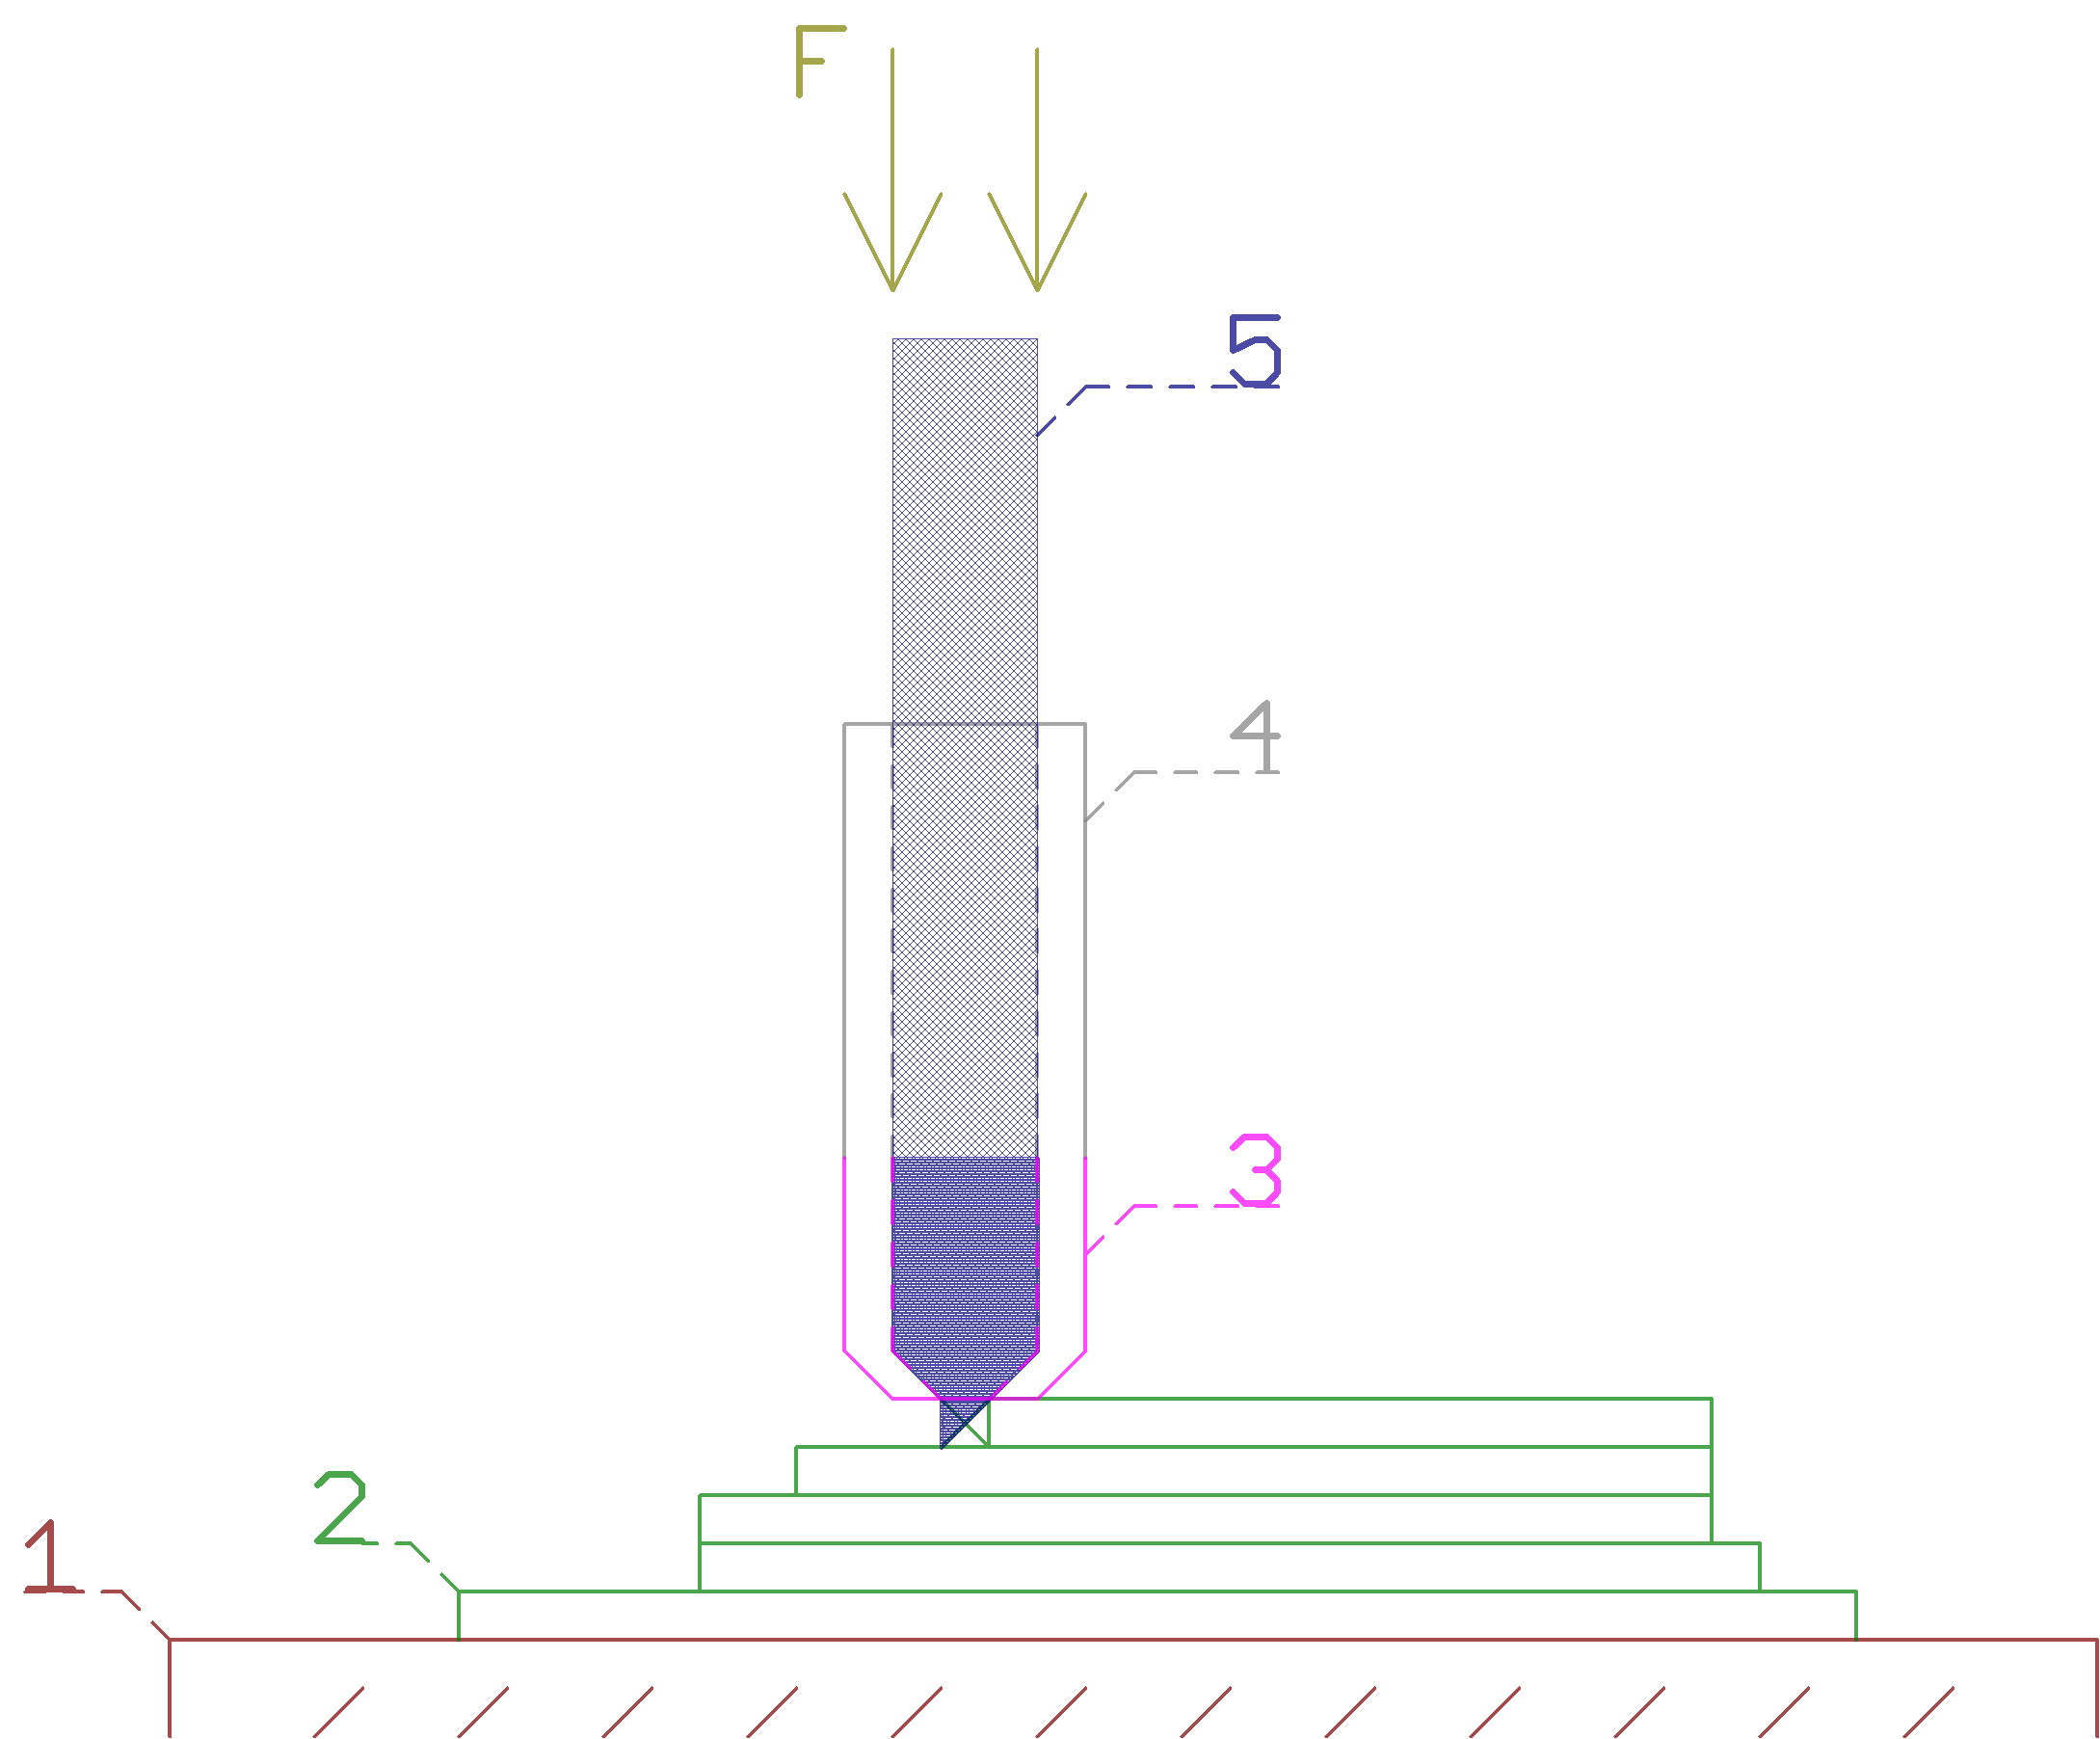
\includegraphics[width=7.5cm]{pics/fdm}
\caption{Princip technologie FDM. 1 - Tisková podložka, 2 - Již hotové vrstvy výsledného objektu, 3 - Horká zóna trysky, 4 - Tryska, 5 - Filament, F - Vtlačovací síla}
\end{center}
\end{figure}


\subsection{Vlastnosti technologie}
3D tisk, podobně jako jiné technologie má specifické vlastnosti, které ovlivňují charakter výsledného produktu. Ovlivněných vlastnostností je velmi mnoho, pro naši aplikaci se zaměříme na dielektrické (chceme vědět jaké bude mít výsledný produkt dielektrické vlastnosti, abychom ho byly schopni popsat, navrhovat a simulovat) a mechanické (produkt musí být možno pevně a stabilě ukotvit na pozici, a musí do něj být možno navázat elektromagnetickou vlnu známým způsobem). Je však nutno brát v potaz, že má i celou řadu vlastností, kterých lze využít pro vytvoření složitých struktur, které by nebylo možné jinými technologiemi jednoduše realizovat, například vnitřní uzavřené struktury. Některé z nich jsou zatím pro dostatečně přesné aproximace dosažitelné v reálném časovém horizontu zcela náhodné, jiné zase přímo ovlivňují námi velmi žádané parametry a můžeme je takto řídit.
\subsubsection{Vrstvy}
Pokud budeme uvažovat ideální podmínky (absolutně čisté prostředí bez kontaminace nechtěnými látkami, ideální filament, rovnoměrnou kontrolovanou distribuci tepla, atd...) stále je objekt tvořem z vrstev. Jelikož vždy vrtva, na které se aktuálně nanáší, je dokonce pod teplotou skelného přechodu, pro odstranění deformace vlivem sil jako gravitace, či tepelné roztažnosti, nedojde k dokonalému spojení polymerních řetězců mezi vrtvami. Při laminaci vrstev může také dojít ke kontaminaci produktu, jako například prachovými částicemi či vzduchovými kapsami. Toto se však dá zanedbat jelikož lze snadno stabilizovat okolní prostředí a minimalizovat vliv. 
Hlavní ovlivněné vlastnosti, pro naši aplikaci podstatné, jsou mechanické. Vždy je v ose vrstev rozložení mezne plasticity neuniformní, dochází tedy k plastické deformaci významně v těchto oblastech, což někdy může být problém z důvodu nutnosti splnění možnosti upevnění a realizovatelnosti produktu.
Z dielektrického hlediska tedy nebude ani relativní permitivita uniformně rozložená v jedné ose, vznikne tedy periodická stuktura. Tento vliv by bylo možné omezit buďto zvýšením diskretizačního kroku, tedy omezením počtu rozhraní, což může v jistých případech ovlivňovat vlastnosti celé struktury vzhledem růstu kvantizačního šumu, nebo naopak snížením kroku kdy již bude úroveň šumu blízká nule, což se bohužel negativně projeví na době tisku, to však v některých případech není problém. Výzkum popisu tohoto chování je však předmětem dalším.

\subsubsection{Vnitřní struktury}
Vlivem principu vrstvení je možno vytvářet vnitřní struktury definovaných tvarů, dokonce i selektivně, a takto velmi silně ovlivňovat pro nás důležité parametry.
Mechanické vlastnosti tímto lze slektivně měnit, například zpevněním montážních ovorů v technologickém okolí, což v našem případě není první v pořadí.
Dielektrické vlastnosti jsou tímto však velmi ovlivněny. Technologií je totiž možno vytvářet prakticky jakékoliv struktury uvnitř produktu ve zvolených místech, tedy například vytisknout Luneburgovu či Maxwell fish-eye čočku. Je však ale nutno provést výzkum na toto téma dostatečné podrobrý výzkum, jedná se totiž o skokové změny vlastností. Tyto změny poté vytváří rozhraní, kde dochází odrazům, které zatím modelovat a popsat je velmi komplexní úlohou.

\begin{figure}[h]
\begin{center}
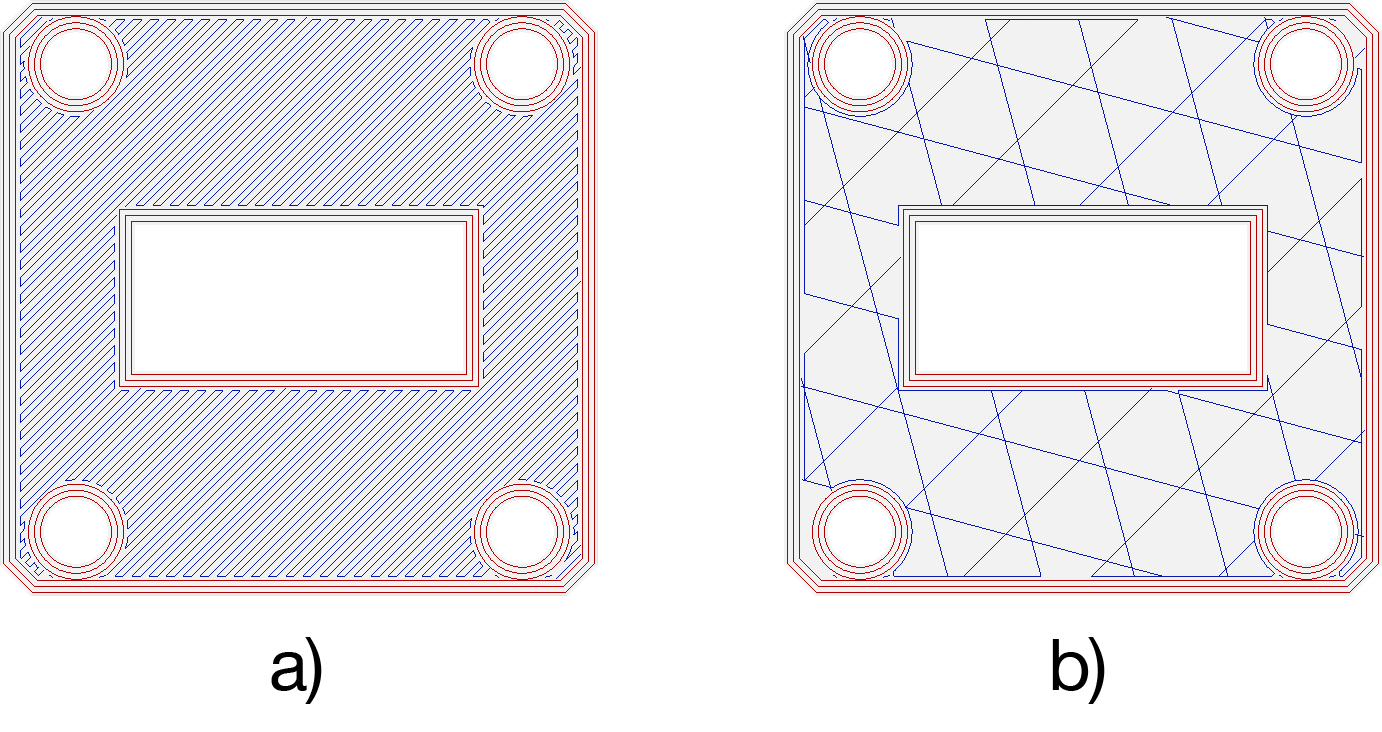
\includegraphics[width=8.5cm]{pics/fillcompare}
\caption{Porovnání různého motivu vrstvy, a) 100\,\% vyplň typem rectilinear, b) 20\,\% vyplnň typem cubic}
\end{center}
\end{figure}

\begin{figure}[h]
\begin{center}
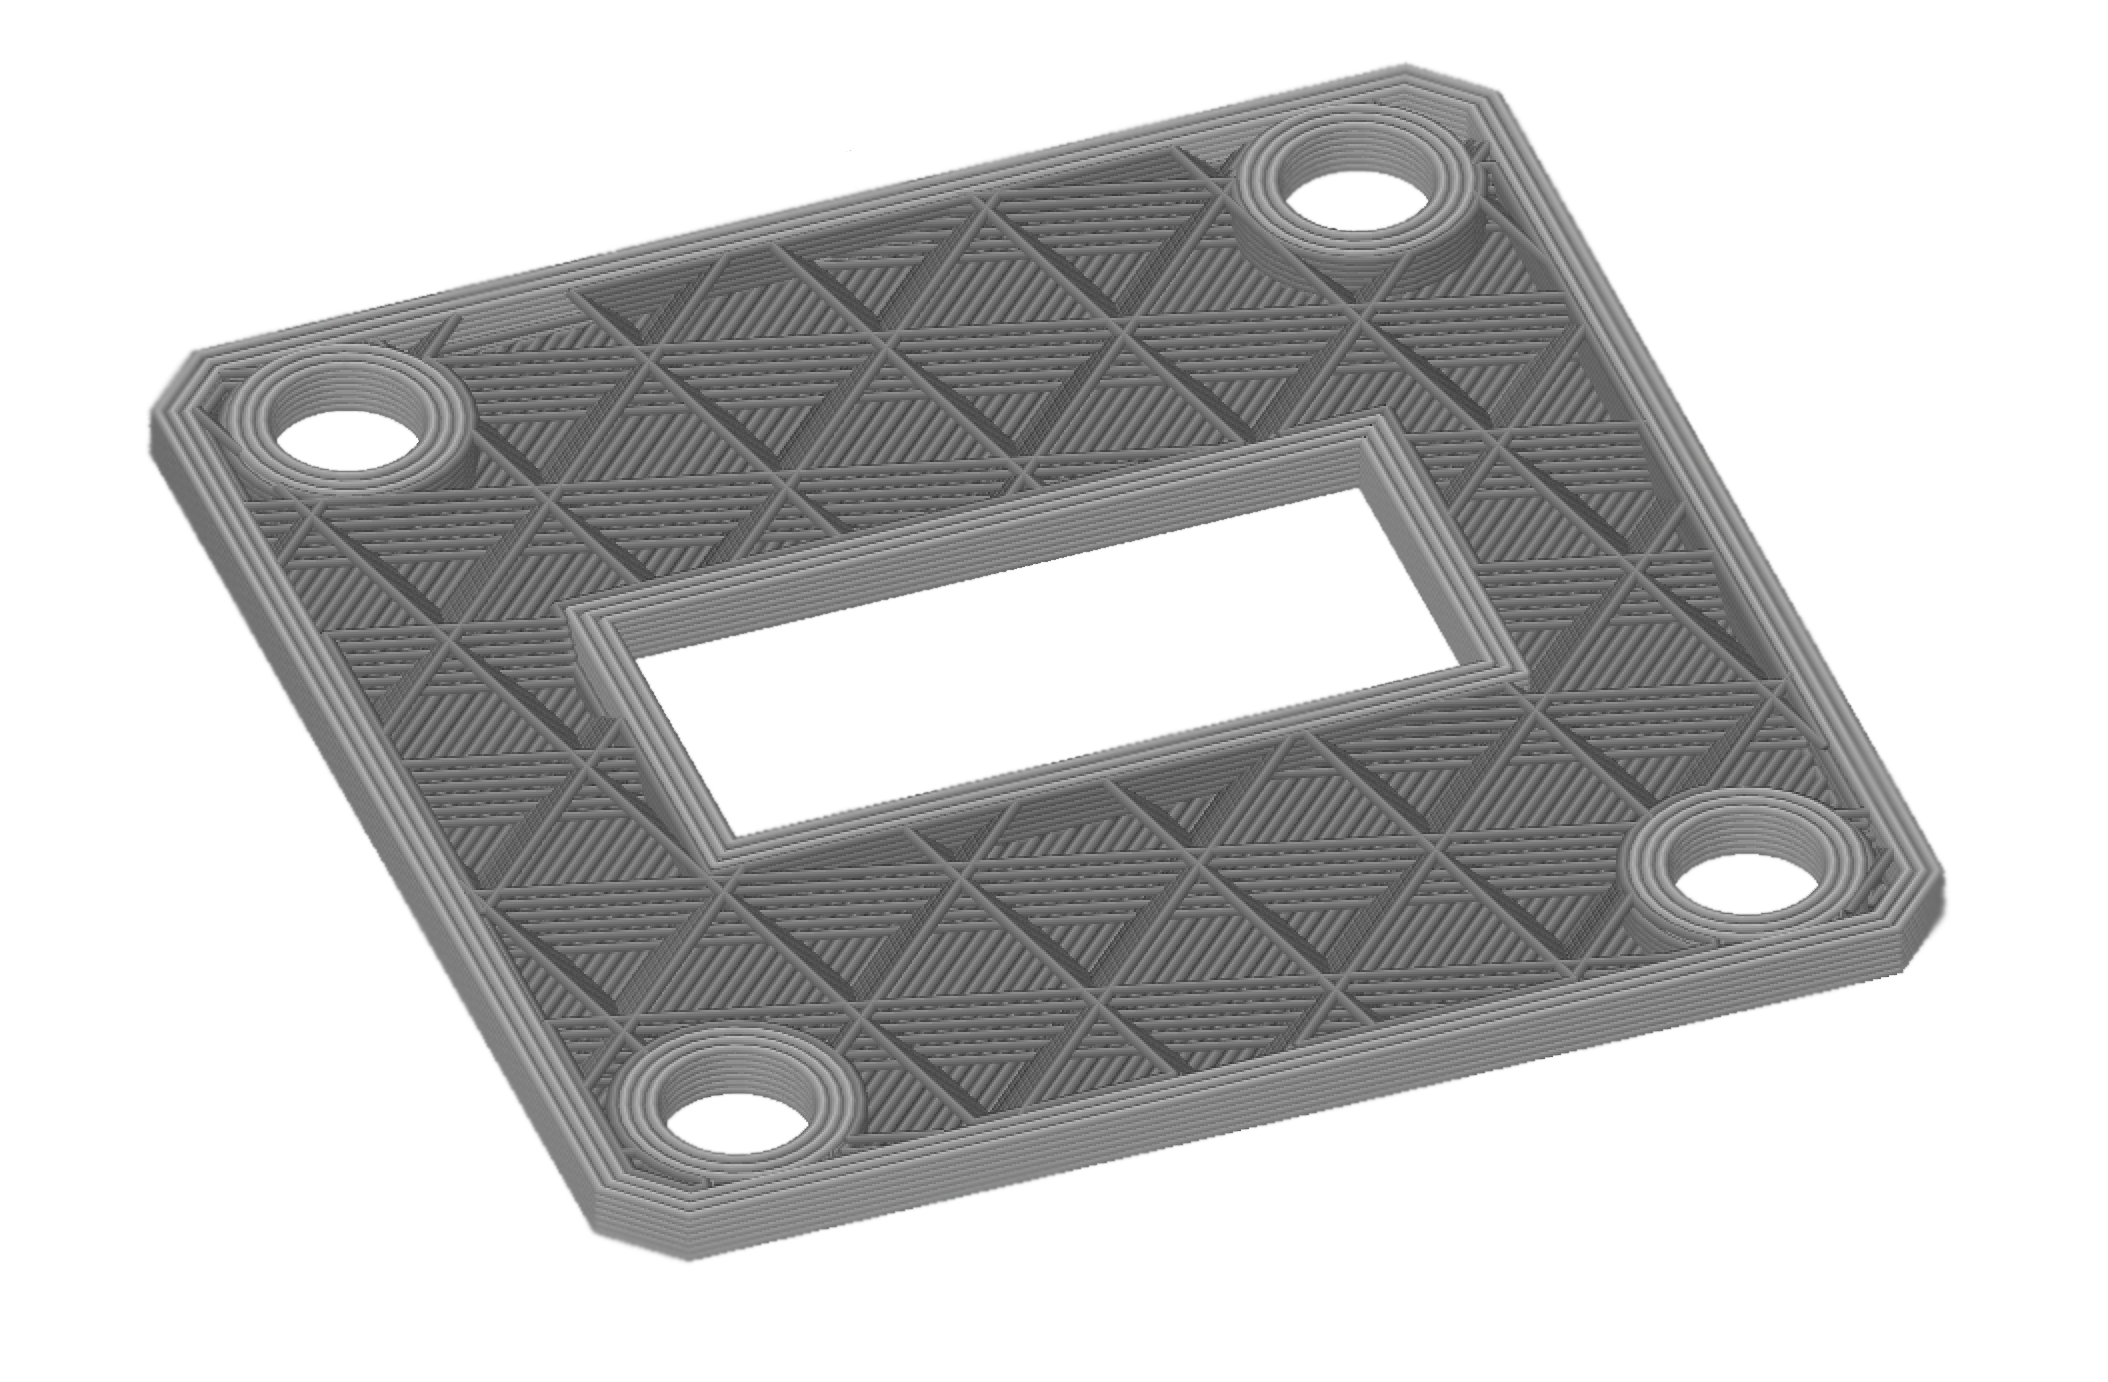
\includegraphics[width=8.5cm]{pics/6layer}
\caption{Náhled vrstev 1-6 struktury s kombinovanou výplní typu rectilinear (první dvě vrstvy) a cubic o rozdílné procentuální výplni}
\end{center}
\end{figure}

\subsection{Materiály využitelné pro vysokofrekvenční techniku}
Termopolymerních materiálů které by se daly využít je celá řada, teoreticky je možné uplatnit velké množství, prakticky však ale vyplývá otázka bezpečnosti, jelikož průchod některých polymerů procesem může uvolňovat nebezpečné látky, či v případě směsí její části. Dále je však nutné brát v potaz i vlastnosti jako tepelná roztažnost 
Mezi nejrozšířenější patří PLA, ABS a PET, tyto materiály však lze uplatnit zejména v čočkách, či dielektrických rezonátorech, jelikož vykazují velmi malou vodivost. Objevují se ale stále nové směsy materiálů jako například PLA s výraznou příměsí grafénových šupin, či měděného prachu které v ideálním případě disponují velmi vysokou vodivostí.

\subsubsection{"Vodivé" materiály}
Jelikož mezi nejrozšířenější materiály patří PLA, které vykazuje výborné zpracovatelské vlastnosti je většina těchno směsí právě na tomto nosiči.
Jako příměs pro vodivé materiály je možno použít teoreticky jakékoliv fragmenty vodivé látky jako třeba měď, stále populárnější je ale grafén, z důvodu jeho vysoké vodivosti způsobené $\pi$ elektrony. Při plnění nosného polymeru je však nutno brát v potaz že při zvyšujícím se podílu plniva se vlastnosti výsledné směsi velmi mění.
Jelikož je pro nás nyní nejvýznamnější elektrická vodivost, je tedy logický cíl maximalizace právě tohoto kritéria. Bohužel se ale stále bude jednat o směs vysoce vodivého materiálu ve velmi nevodivém polymeru, což má dramatický dopad na výsledek. V první řadě ikdyž budeme uvažovat dokonale uniformní rozložení a identické frakce příměsi ve filamentu, vlivem průchodu extrudérem nelze předpokládat, že výsledek bude stejný. Dochází totiž k opětovnému promísení a dokonalý popis celého systému zatím není znám. V druhé řadě je třeba stále brát ohled na zpracovatelnost materiálu a volit správné poměry příměsí, z pravidla 40 - 80\,\%\cite{Dolecek}. Z výše uvedených faktů je bohužel patrné, že výsledný produkt má nezanedbatelné dielektrické vlastnosti.
Ačkoliv se může zdát že tyto materiály nejsou pro naši aplikaci zatím použitelné, stále existuje možnost následného pokovení produktu, kde tyto vlastnosti výrazně zjednoduší proces.

\section{Trychtýřová anténa}
Trychtýřová anténa patří mezi základní anténní struktury využívané jak samostatně, tak ve formě ozařovačů reflektorových antén, či v kombinaci s anténní čočkou. Těchto struktur existuje několik druhů, v našem případě se ale zaměříme na nejpoužívanější, tedy pyramidální trychtýřovou anténu.
Tento typ antény byl zvolen zejména kvůli své jednoduchosti a požadavkům na technologii výroby.

\subsection{Základní princip}
Trychtýřová antená není nic jiného, než postupně se rozšiřující ústí vlnovodu v daných směrech. V případě pyramidálního trychtýře dochází k otevření jak v $E$, tak $H$ rovině. Postupné otevření trychtýře lze považovat za impedanční transformátor zajišťující, v ideálním případě bezodrazné, vyvázání vlny do volného prostoru v definovaném pásmu.
Základní parametry jsou vyobrazeny na obrázku \ref{fig:horn},\ref{fig:hornEH}.

\begin{figure}[h]
\begin{center}
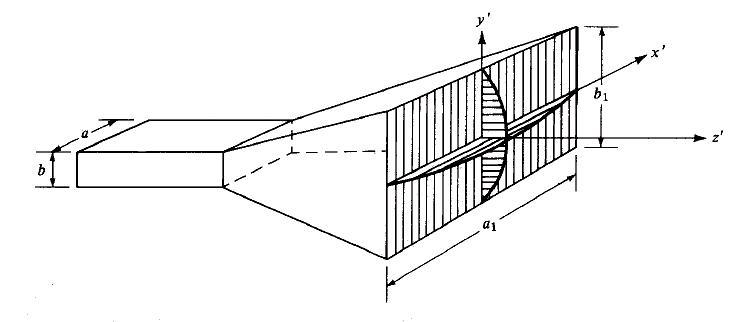
\includegraphics[width=9.5cm]{pics/horn}
\caption{Pyramidální trychtýřová anténa \cite{ConstantineTheory}}
\label{fig:horn}
\end{center}
\end{figure}

\begin{figure}[h]
\begin{center}
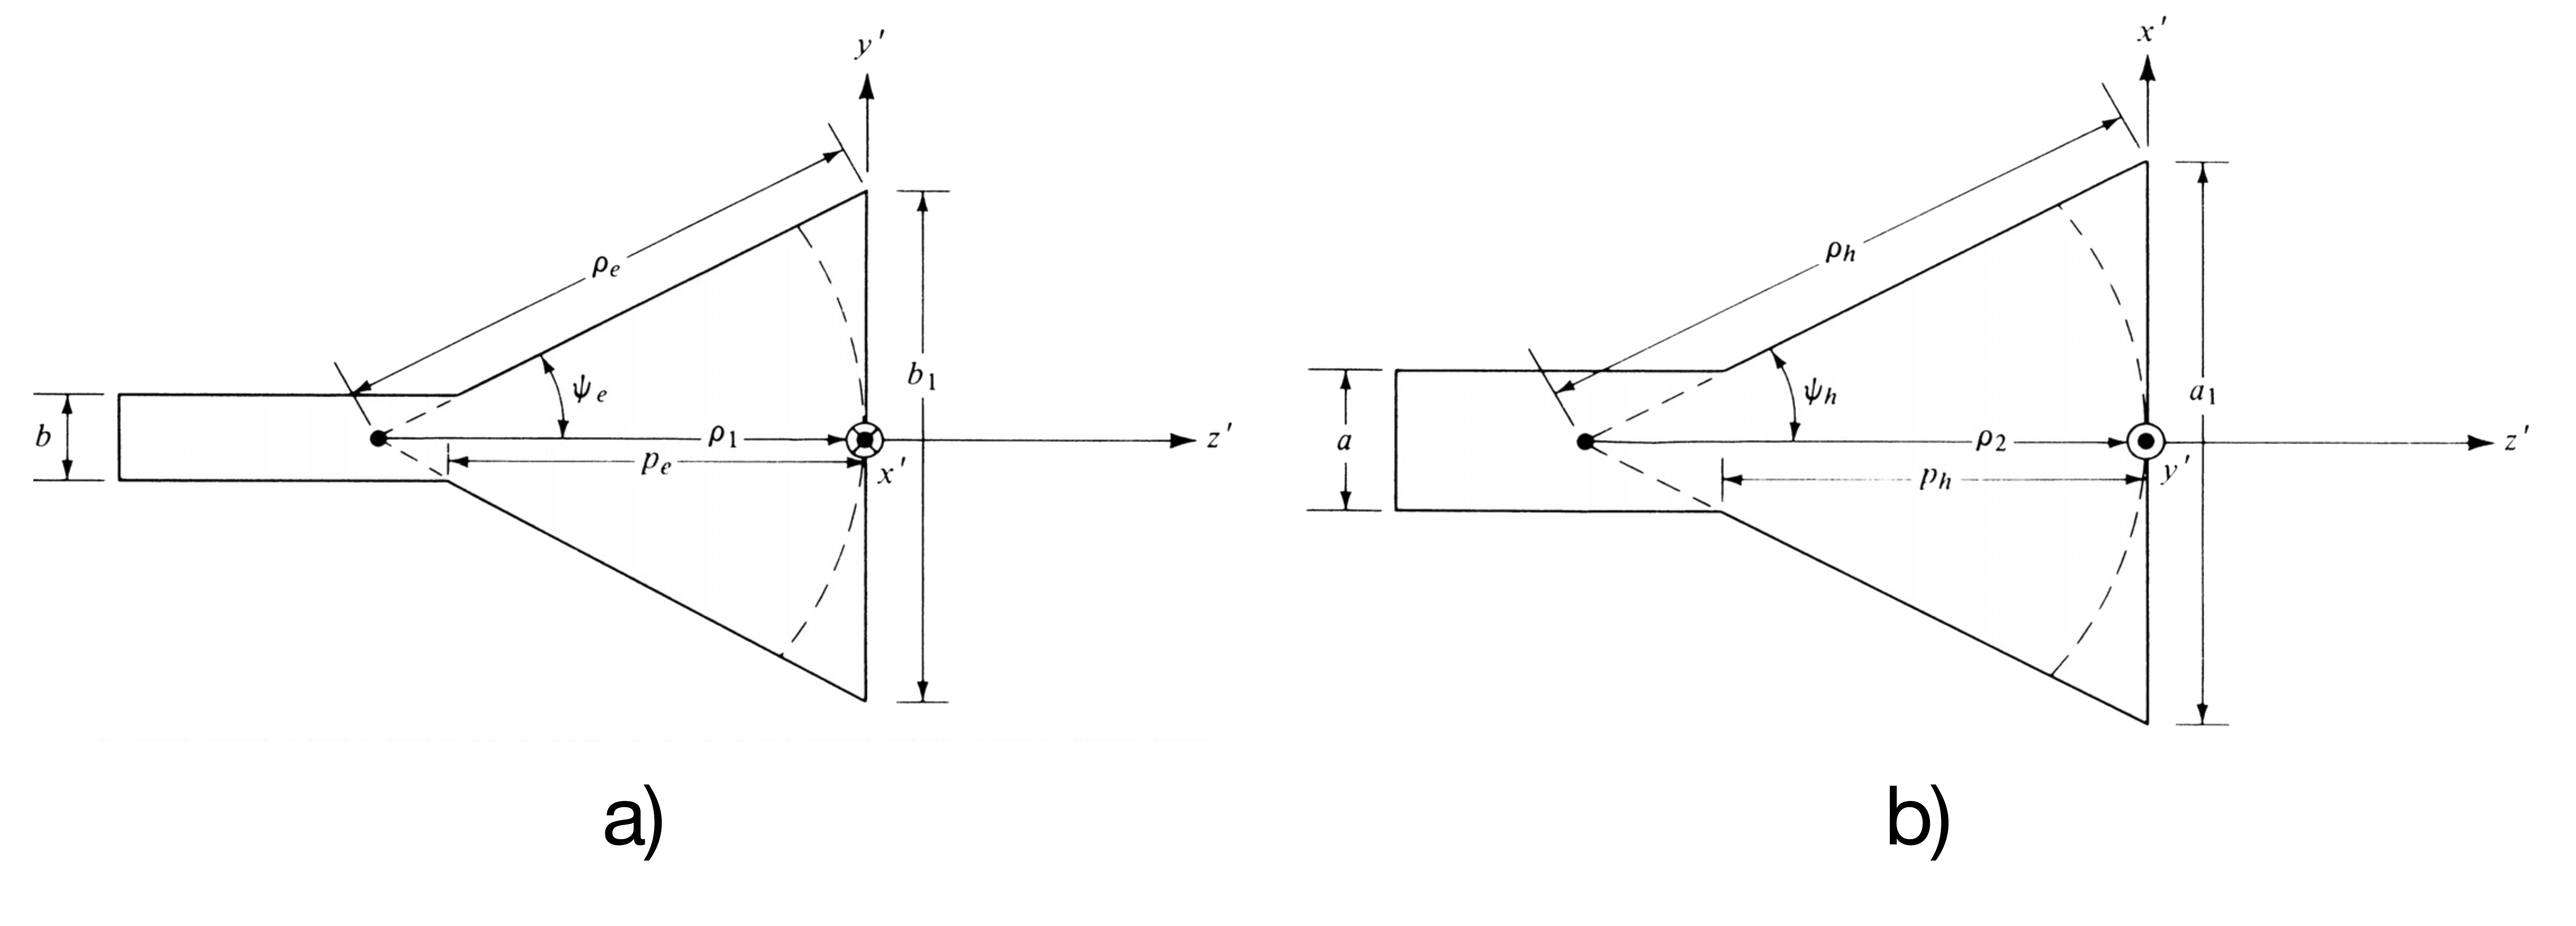
\includegraphics[width=15cm]{pics/hornEH}
\caption{Pyramidální trychtýřová anténa v řezu a)E-roviny, b)H-roviny \cite{ConstantineTheory}}
\label{fig:hornEH}
\end{center}
\end{figure}
\begin{itemize}
\item $a, b$ - Rozměry vlnovodu
\item $a_1, b_1$ - Rozměry ústí trychtýře
\item $p_1, p_2$ - Vzdálenost vrcholu trychtýře od ústí v E a H rovině
\item $x', y'$ - E-rovina, H-rovina
\item $z'$ - Směr Poyntingova vektoru
\item $\rho$ - Délka stěny trychtýře
\item $p$ - Délka trychtýře
\item $\psi$ - Úhel otevření
\end{itemize}

\subsection{Charakterizace struktury}


\subsubsection{Směrovost a zisk}
Směrovost charakterizuje strukturu z hlediska poměru intenzit vyzářeného výkonu struktury do určitého směru, ku celkovému vyzářenému výkonu do celého prostoru. Jde tedy o schopnost antény "směrovat" výkon do určitého směru. Toto však z principu reciprocity paltí i opačně, tedy pro přijatý výkon. Na základě tohoto lze definovat maximální směrovost antény \ref{eq:hornD}.

\begin{equation}
D_p/dB = 10*[1.008+\log_{10}({\frac{a_1 * b_1}{\lambda^2}})]
\label{eq:hornD}
\end{equation}

\renewcommand{\figurename}{Obrázek}
Zisk antény \ref{eq:hornG} je však pro aplikace zajímavějším parametrem, jelikož zahrnuje i ztráty vyzařovací účinností $\eta_r$.
\begin{equation}
G_{dB} = D_{dB} - \eta_{r(dB)}
\label{eq:hornG}
\end{equation}

\subsubsection{Fázová chyba}
Jelikož při vyvazování vlny z vlnovodu do volného prostředí dochází k transformaci vlny rovinné na kulovou. Z této skutečnosti plyne, že na rozhraní ústí trychtýře bude existovat oblast, kde se střed vlny bude nacházet právě na rozhraní, ale její okraje stále uvnitř. Tento rozdíl se nazývá fázová chyba a vede k deformaci směrové charakteristiky a snížení směrovosti. Pro minimalizaci této chyby je vhodné, aby úhel otevření trychtýře byl co nejmenší, nicméně je však ale nutno brát v potaz, že tímto narůstá jeho odélka a zároveň i náročnost realizace.
\begin{figure}[h]
\begin{center}
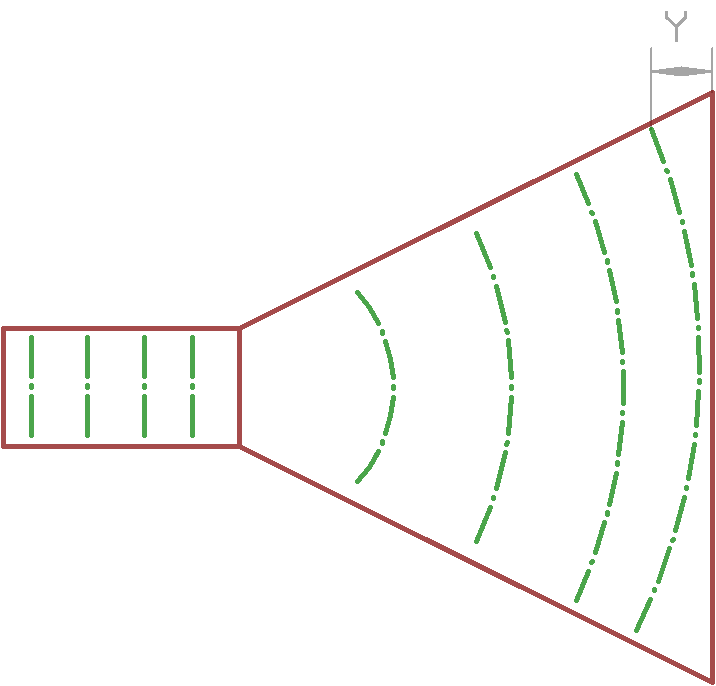
\includegraphics[width=6.5cm]{pics/hornErr}
\caption{Znázornění fázové chyby $Y$}
\label{fig:HornErr}
\end{center}
\end{figure}

\begin{figure}
\begin{tikzpicture}[scale=1.4]
\begin{axis}[
    xlabel={Angle /},
    ylabel={Amplitude /\,dB},
    minor tick num=10,
    minor grid style={gray!25},
  	major grid style={black!50},
  	xmin=-180,xmax = 180,
  	%ymin=-120, ymax=-60,
    grid=both
]
\addplot [no markers, thick, blue] table [col sep=tab, y=AeOpt] {hornSim.dat};
\addplot [no markers, thick, green] table [col sep=tab, y=Ae180] {hornSim.dat};
\addplot [no markers, thick, orange] table [col sep=tab, y=Ae140thin] {hornSim.dat};
\legend{228\,mm,180\,mm,140\,mm};
\end{axis}
\end{tikzpicture}
\caption{Řezy směrových charakteristiky v E rovině pro různé úhly otevření pyramidálního trychtýře}
\label{fig:HornLenDep}
\end{figure}

\newpage
\section{Anténní čočky}
Podobně jako v optice, i zde lze použít čočku, jelikož světlo má z důvodu duality i charakter vlny. Existuje tedy celá řada různých realizací čoček, lze je rozdělit do dvou základních kategorií:
\begin{itemize}
\item Zpomalovací, neboli dielektrické
\item Urychlující, neboli kovové
\end{itemize}

\subsection{Základní princip}
Hlavním úkolem čočky je kolimovat paprsek, neboli šnížit rozbíhavost, v případě anténní domény transformovat kulovou vlnu na rovinnou. Jak můžeme vidět na obrázku \ref{fig:hornLens}, kde:
\begin{itemize}
\item $1$ - Trychtýřová anténa
\item $2$ - Vystupující kulová vlna z trychtýře
\item $3$ - Anténní plano-konvexní čočka
\item $4$ - Výsledná rovinná vlna
\item $X$ - Parametr kulovitosti vstupní vlny
\item $X'$ - Parametr kulovitosti výstupní vlny
\end{itemize}
\begin{figure}[h]
\begin{center}
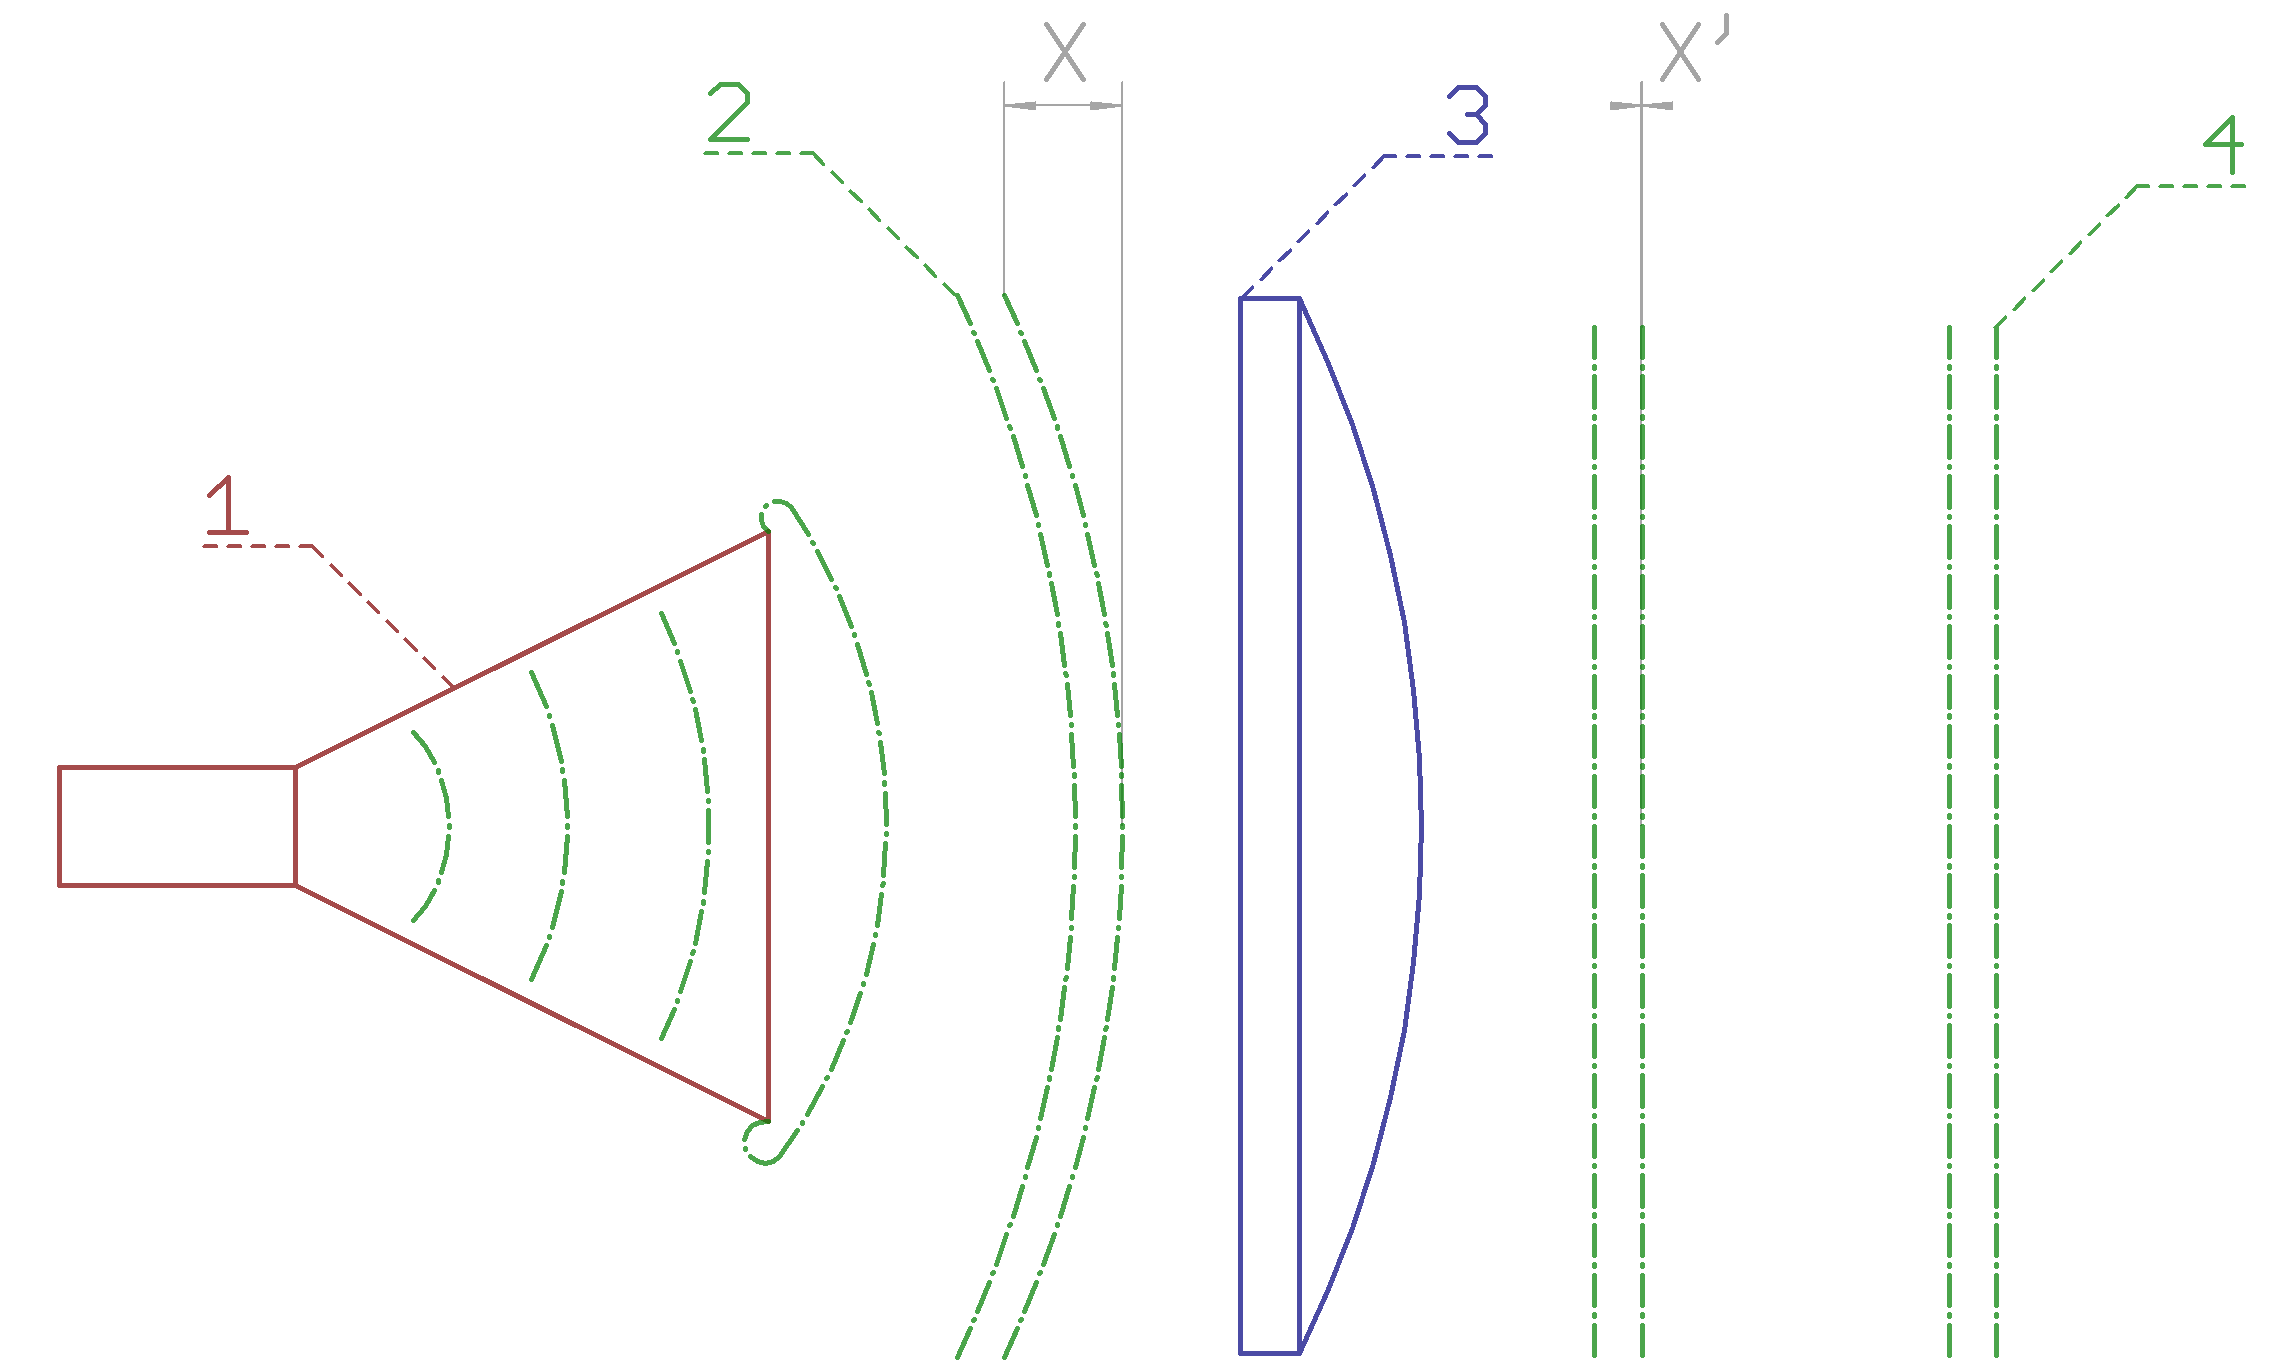
\includegraphics[width=9.5cm]{pics/lens}
\caption{Princip anténní čočky}
\label{fig:hornLens}
\end{center}
\end{figure}
Pro zajištění této funkce je však ale nutno, aby anténní čočka měla rozdílnou relativní permitivitu $\epsilon_r$ než okolní prostředí, ve kterém se vlna šíří. Touto podmínkou je způsobeno zpomalení, nebo zrychlení, vlny a následné kolimaci. Z čehož plyne již výše uvedené rozdělení čoček, viz obrázek \ref{fig:LensTypes}.
\begin{figure}[h]
\begin{center}
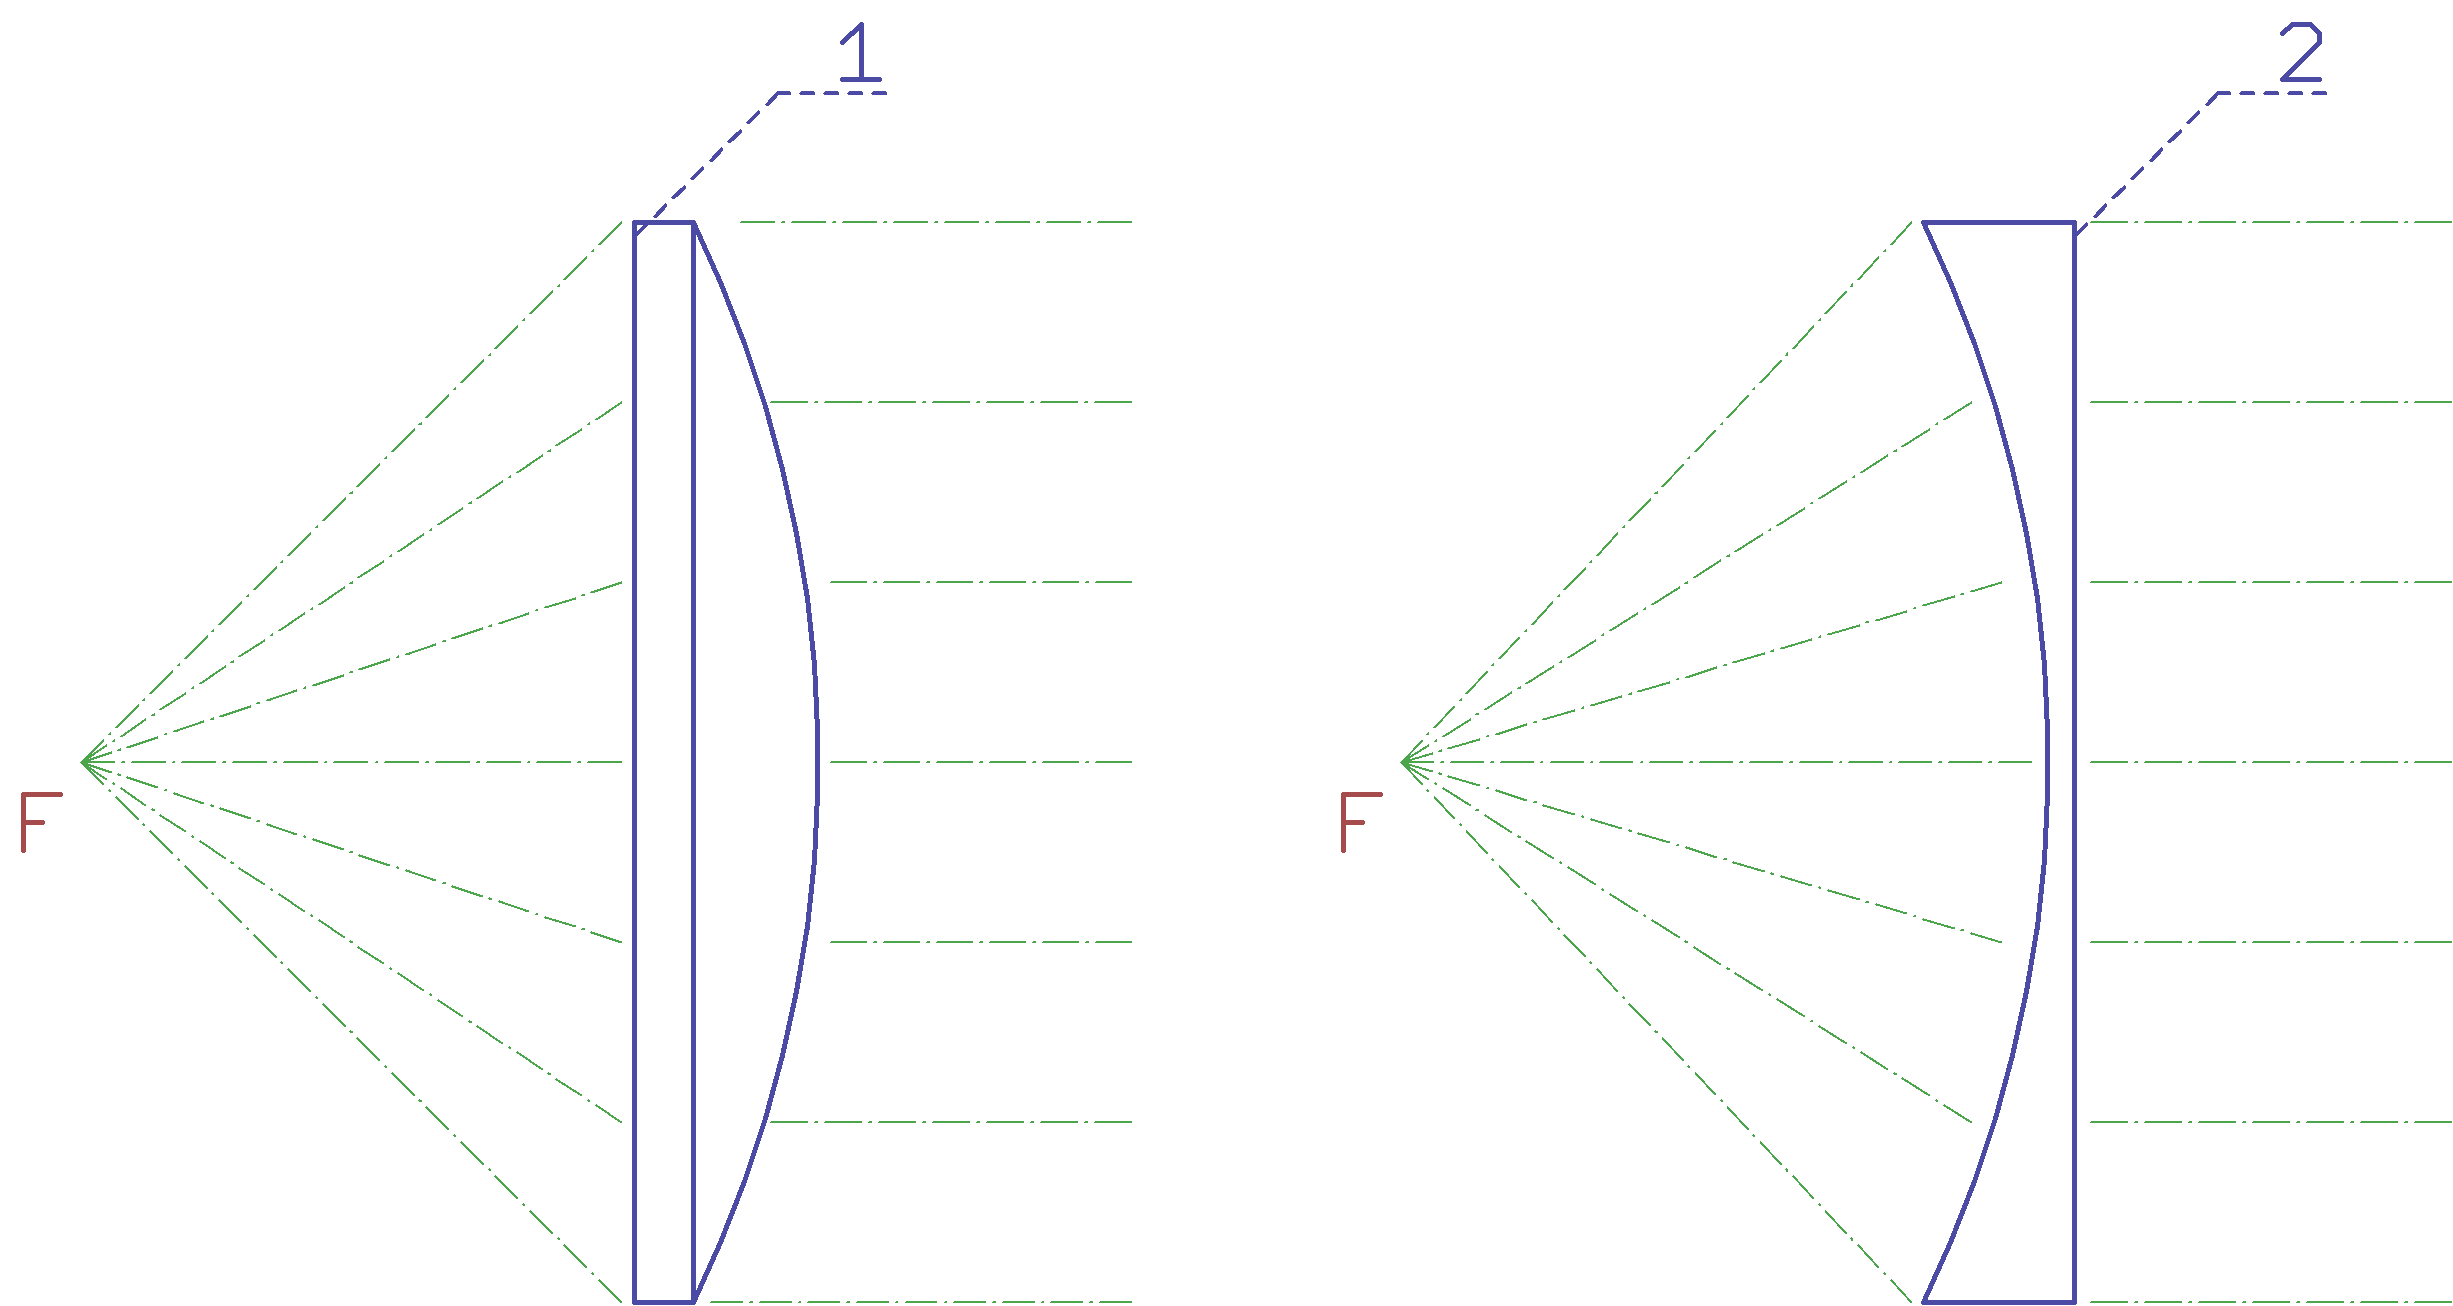
\includegraphics[width=9.5cm]{pics/lenstypes}
\caption{Typy anténních čoček. 1 - Zpomalující, 2 - Zrychlující}
\label{fig:LensTypes}
\end{center}
\end{figure}

\section{Extrakce dielektrických parametrů}
Znalost dielektrických parametrů je klíčová pro návrh vlastních strukur, zejména anténních čoček.
Pro většinu materiálů jsou tyto parametry již známé, nicméně pokud se rozhodneme strukturu realizovat technologií 3D tisků, vstypuje do tohoto mnoho dalších proměnných které mohou výrazně ovlivnit výsledné parametry produktu, ať už v prospěch, či naopak.
Pro získání těchto parametrů lze použít například proces integrovaný v CST MW studio, který lze papsat blokovým schématem na obrázku \ref{fig:ExtractBlock}
\begin{figure}[h]
\begin{center}
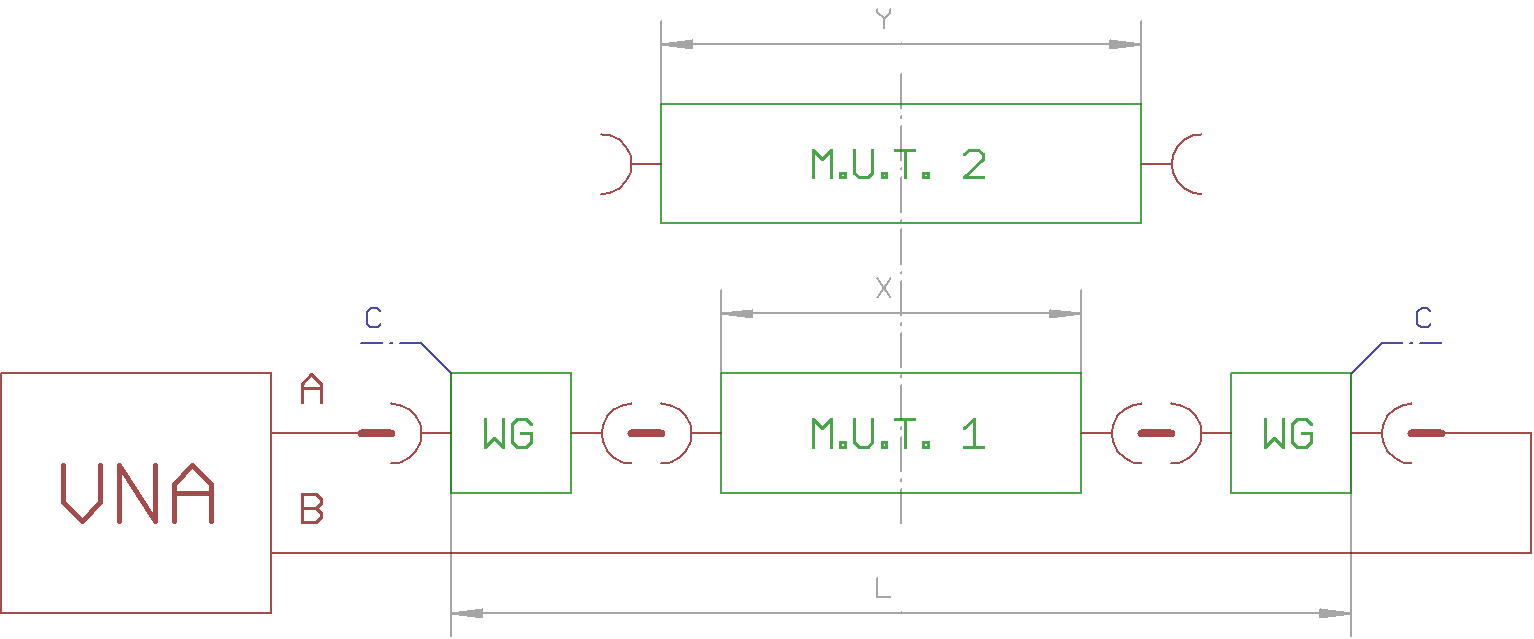
\includegraphics[width=9.5cm]{pics/ExtractBlock}
\caption{Blokové schéma transmisní/reflexní extrakce dielektrických parametrů}
\label{fig:ExtractBlock}
\end{center}
\end{figure} 
\subsection{Princip extrakce}
Extrakce parametrů spočívá ve změření přenosu mezi kanály $A$ a $B$ vektorového analyzátoru pro dva geometricky odlišné vzorky materiálu, jehož parametry chceme extrahovat. Jelikož v systému dojde ke změně pouze rozměru neznámého materiálu, tak na základě rozdílného přenosu jsme schopni z naměřených dat extrahovat dielektrické parametry jako relativní permitivitu $\epsilon_r$ a ztrátový činitel $tg_\delta$.

%% This is an example first chapter.  You should put chapter/appendix that you
%% write into a separate file, and add a line \include{yourfilename} to
%% main.tex, where `yourfilename.tex' is the name of the chapter/appendix file.
%% You can process specific files by typing their names in at the 
%% \files=
%% prompt when you run the file main.tex through LaTeX.
\chapter{Návrh}

\section{Trychtýřová antnéna}

\section{Anténní čočka}

\section{Extrakce dielektrických parametrů}
%% This is an example first chapter.  You should put chapter/appendix that you
%% write into a separate file, and add a line \include{yourfilename} to
%% main.tex, where `yourfilename.tex' is the name of the chapter/appendix file.
%% You can process specific files by typing their names in at the 
%% \files=
%% prompt when you run the file main.tex through LaTeX.
\chapter{Realizace}

Vlastní realizace struktury není pouhé vygenerování dat pomocí standartních dostupných nastavení, ovšem brzy bude, následný tisk, případný post-processing, a aplikace.

Jelikož se vlastnosti zejména vodivých filamentů zásadně liší od běžně dostupných, je patrné, že bude nutno proces dostatečně upravit pro úspěšné dokončení tisku, jeho opakovatelnosti a následné použitelnosti produktu. Podobně jako v případě post-processingu v podobě pokovení.

Naopak anténní čočka a vzorky pro extrakci parametrů lze realizovat standartním způsobem a je pouze otázkou časové náročnosti procesu a voblou správného materiálu.

\section{3D tisk}
Realizace veškerých struktur v této práci byla pomocí technologie 3D tisku FDM, kterou jsme si již vysvětlili v kapitole 1. Opět však je možnost zvolit nepřeberné množství tirkáren kterou jsou čím dál více dostupné, v tomto případě se jednalo o Original Prusa i3 MK2. Toto zařízení patří mezi nejpoužívanější stolní 3D tiskárny na světě \cite{3Dhubs} a existuje široká škála již před připravených, řádně otestovaných, tiskových nastavení ze které výrazně urychlí případné ladění pro specifický materiál.

\subsubsection{Trychtýřová anténa}
Jelikož bylo primárním cílem možnost použití produktu přímo bez post-processignu, je tedy nezbytné volit vodivé filamenty. Tyto materiály, jak již víme mají výrazně odlišné vlastnosti od jejich nosičů.

Pro námi navrženou anténu byly použity následující filamenty:
\begin{itemize}
\item Electrifi Conductive 3D Printing Filament
\item F-Electric Filament
\item Blackmagic 3D Conductive Graphene Filament
\item MKF Filament MKF-ABS F1.75 černá / VODIVÁ
\end{itemize}

Veškeré použité filamenty jsou na nosiči PLA, s vyjímkou MKF-ABS. Jako příměs jsou použity grafenové fragmenty (Blackmagic), uhlíkové nanotrubky (F-electric) a měďěné částice (Electrifi). Bohužel u materiálu MKF nebylo možné s dostatečnou přesností určit příměs jelikož výrobce tento údajneposkytuje. Podobná situace poté však ale platí i procentuální podíl příměsí, které jsou buďto tajné, či neznámé pro všechny testované vzorky.

Z hlediska vodivosti, tedy nejlepšího kandidáta na použití při realizaci dle udávaných parametrů (byly-li dostupné) je jednoznažně Electrify, který udává $16667\,S/m$. Nicméně je velmi důležitá jeho náročnost na tiskový proces vlivem velkého procenta mědi, která akumuluje teplo a značně prodlužuje zchlazení objektu pod teplotu skelného přechodu způsobující následnou deformaci tisknutého produktu vlivem gravitace.

Dalším významným faktorem filamenty Electrifi je jeho cena, $199.53\,CZK$/m. Pokud bychom tedy chtěli realizovat námi navržený trychtýř, bylo by nezbytné použít téměř 27\,m, celkem tedy $5 387\,CZK$ za předpokladu 100\,\% úspěšnosti realizace.

Jako reálnější materiály poté vychází F-electric, s vodivostí $133.33\,S/m$ a cenou $25.73\,CZK$/m, $694.71\,CZK$ za trychtýř, či Blackmagic, s vodivostí $166.67\,S$ a cenou $43.2\,CZK$/m, $1 166.4\,CZK$ za trychtýř, které vykazují výrazně vhodnější parametry pro tisk.

Před vlastní generací dat je však nutno vyrvořit profil charakterizující materiál z hlediska teplot, rychlosti procesu, chalzení, a ostatních parametrů. Pro získání prvnotního návrhu nastavení lze pouze převzít doporučené hodnoty výrobcem, nicméně ne vždy toto musí platit! Jelikož neexistuje jednotný standart pro 3D tiskrány typu: tiskový povrch, geometrie trysky, mechanika extruderu, a další, bude pravděpodobné že toto nastavení ve finální podobě bude odlišné.

\begin{figure}[h]
\begin{center}
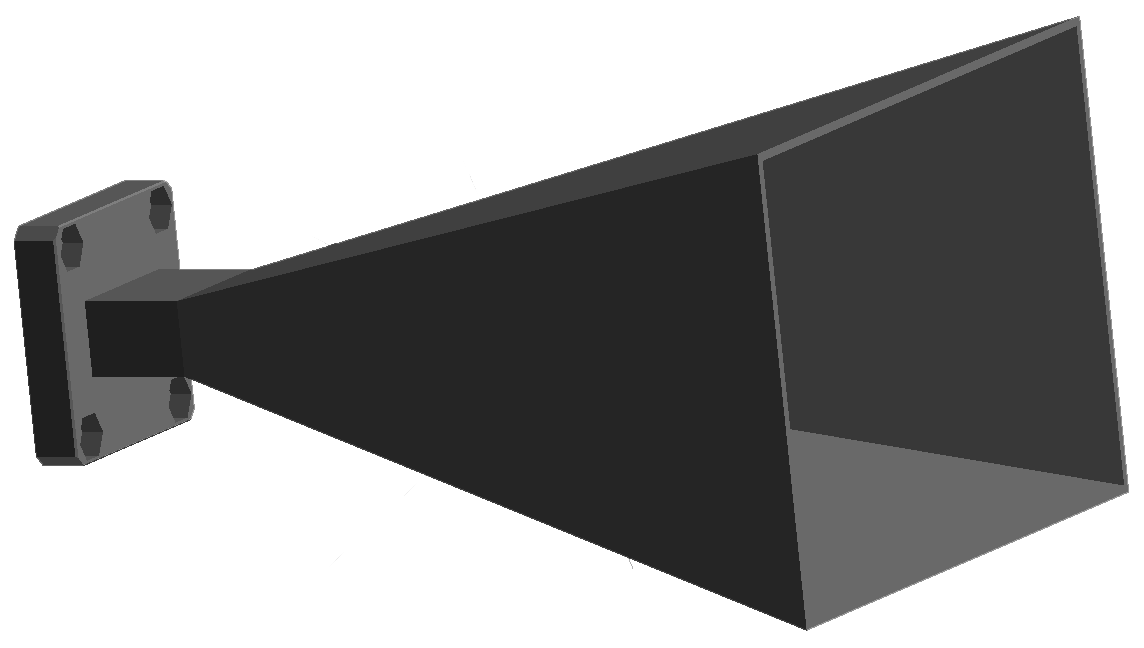
\includegraphics[width=9.5cm]{pics/HornFinal}
\caption{Výsledný model trychtýřové antény včetně příruby na vlnovod realizovaný technologií 3D tisku za použití F-electric filamentu}
\label{fig:HornRealFe}
\end{center}
\end{figure}

Bohužel však při realizaci dalších struktur docházelo k významným komplikacím znemožňující další produkci, zejména k ucpavání trysky \ref{fig:HornFail}.

K těmto skutečnostem pravděpodobně vedlo nadměrné hromadění příměsí v místě zužení trysky způsobující zúst mechanického odporu a nároků na potřebnou sílu k jeho překonání. Vlivem nízké mechanické soudržnosti materiálu a křehkosti způsobeno vysokým procentem plnění poté dochází k prokluzování podávacího mechanismu extruderu a následného výpadku extruze. Další pravděpodobnou příčinou mohl být vlastní průměr filamentu, který pokud je mimo specifikaci ($\pm0.05\,mm$) může dojít k podobné situaci jelikož ne vždy je možné protáhnout předmět větší než rozměry otvoru. 

Tyto komplikace byly částečně eliminovány použitím trysky $D_{nozzle} = 0.6\,mm$, avšak problémy stále přetrvávali a proces byl velmi nespolehlivý a neopakovatelný. Možné další principy eliminace mohou být realizovány například úpravou mechanické části extruderu, která by měla výrazně větší styčnou plochu podávacího mechanismu s filamentem pro možnost vyvinou vyšší tlačnou sílu.

\begin{figure}[h]
\begin{center}
\includegraphics[width=9.5cm]{pics/HornFail}
\caption{Důsledek ucpavání trysky v průběhu tisku modelu}
\label{fig:HornFail}
\end{center}
\end{figure}


\subsubsection{Anténní čočka}
Realizace anténní čočky je v porovnání s předchozím případem velmi zjednodušena z důvodu zvolení zpomalujícího typu, tedy použití dielektrického, nikoliv vodivého, materiálu.

Pro správnou funkci čočky a maximálnímu přiblížení se simulovaných modelů je důležité při generování dat pro technologický proces použít správný typ vnitřní struktury pro zajištění 100\.\% podílu dielektrického materiálu.

Pokud toto nebude při realizaci dodrženo, vlivem nehomogenního prostředí pro šíření vlny, obsahující mnoho velmi ostrých rozhraní vzduch/dielektrikum, způsobí velmi odlišné chování a pro jeho dostatečný popis je třeba k téro struktuře přistupovat jako k metamateriálu.



\section{Pokovení}



\section{Měření parametrů}

\begin{figure}
\begin{tikzpicture}[scale=1.4]
\begin{axis}[
    xlabel={Angle /\,$^\circ$},
    ylabel={Amplitude /\,dB},
    minor tick num=10,
    minor grid style={gray!25},
  	major grid style={black!50},
  	xmin=-180,xmax = 180,
  	ymin=-120, ymax=-60,
    grid=both
]
\addplot [no markers, thick, blue] table [col sep=tab, y=Ae-graph] {horn.dat};
\addplot [no markers, thick, red] table [col sep=tab, y=Ae-emi] {horn.dat};
\addplot [no markers, thick, green] table [col sep=tab, y=Ae-lens] {horn.dat};
\end{axis}
\end{tikzpicture}
\caption{Řez naměřené vyzařovací charakteristiky realizovaného trychtýře z materiálu F-electric v E rovině}
\end{figure}

\begin{figure}
\begin{tikzpicture}
\begin{axis}[
    xlabel={Angle /\,$^\circ$},
    ylabel={Amplitude /\,dB},
    minor tick num=10,
    minor grid style={gray!25},
  	major grid style={black!50},
  	xmin=-180,xmax = 180,
  	ymin=-120, ymax=-60,
    grid=both
]
\addplot [no markers, thick, blue] table [col sep=tab, y=Ah-graph] {horn.dat};
\addplot [no markers, thick, red] table [col sep=tab, y=Ah-emi] {horn.dat};
\addplot [no markers, thick, green] table [col sep=tab, y=Ah-lens] {horn.dat};
\end{axis}
\end{tikzpicture}
\caption{Řez vyzařovací charakteristiky v H rovině}
\end{figure}




%% This is an example first chapter.  You should put chapter/appendix that you
%% write into a separate file, and add a line \include{yourfilename} to
%% main.tex, where `yourfilename.tex' is the name of the chapter/appendix file.
%% You can process specific files by typing their names in at the 
%% \files=
%% prompt when you run the file main.tex through LaTeX.
\chapter{Závěr}



\begin{thebibliography}{9}

\bibitem{ModernLens}
  John Thornton,
  Kao-Cheng Huang,
  MODERN LENS ANTENNAS FOR COMMUNICATIONS ENGINEERING,
  Wiley,
  IEEE PRESS,
  2013.

\bibitem{Dolecek}
  Josef Doleček,
  Fillamentum,
  Parzlich s.r.o.,
  Konzultace na téma výroby filamentů,
  2016.

\bibitem{ConstantineTheory}
  Constantine A. Balanis,
  Antenna theory analysis and design,
  Wiley,
  4th edition,
  2016.

\bibitem{3Dhubs}
  https://www.3dhubs.com/trends,
  2017.

\bibitem{EMIdata}
  https://www.gme.cz/data/attachments/dsh.749-035.1.pdf,
  Datasheet EMI 35 spray,
  2007.

\bibitem{Electroforming}
  http://www.electroforming.cz/cs/technologie,
  Elektroforming, popis technologie 
  2017.
  

\end{thebibliography}

\newpage

\listoffigures

\newpage

\listoftables

% $Log: abstract.tex,v $
% Revision 1.1  93/05/14  14:56:25  starflt
% Initial revision
% 
% Revision 1.1  90/05/04  10:41:01  lwvanels
% Initial revision
% 
%
%% The text of your abstract and nothing else (other than comments) goes here.
%% It will be single-spaced and the rest of the text that is supposed to go on
%% the abstract page will be generated by the abstractpage environment.  This
%% file should be \input (not \include 'd) from cover.tex.
\thispagestyle{empty}
\chapter*{Seznam použitých symbolů a zkratek}
\thispagestyle{empty}
\itab{3D} \tab{} \tab{3-rozměrné}\\*
\itab{LED} \tab{} \tab{Světlo emitující dioda}\\*
\itab{CD} \tab{} \tab{Kompaktní disk}\\*
\itab{VNA} \tab{} \tab{Vector network analyzer}\\*
\itab{ABS} \tab{} \tab{Acrylonitrile butadiene styrene}\\*
\itab{PLA} \tab{} \tab{Polylactic acid}\\*
\itab{PET} \tab{} \tab{Polyethylene terephthalate}\\*
\itab{D.U.T.} \tab{} \tab{Device under test}\\*


%\include{99-add-safety}

\chapter{Obsah přiloženého CD}
Na přiloženém CD jsou uloženy v adresáři:
\begin{itemize}
\item \textbf{man-data} všechna výrobní data použita při řešení práce.
\item \textbf{text} je uložena tato práce ve formátu *.pdf.
\end{itemize} 


\thispagestyle{empty}
\null\newpage

%%\include{biblio}
\end{document}

